
%(BEGIN_QUESTION)
% Copyright 2013, Tony R. Kuphaldt, released under the Creative Commons Attribution License (v 1.0)
% This means you may do almost anything with this work of mine, so long as you give me proper credit

En tank som inneholder 4m med væske utgjør et hydrostatisk trykk på et manometer montert i bunn av tanken. 

$$\includegraphics[width=8cm]{i02822x01.eps}$$

Regn ut det hydrostatiske trykket maometeres viser i kPa

\vskip 10pt

$P$ = \underbar{\hskip 50pt} kPa

\vskip 10pt

\underbar{file i02822}
%(END_QUESTION)





%(BEGIN_ANSWER)

$P$ = \underbar{\bf 30.11} kPa
 
%(END_ANSWER)





%(BEGIN_NOTES)


%INDEX% Physics, static fluids: hydrostatic pressure

%(END_NOTES)


